\chapter{Dedičnosť}
\label{sect:dedicnost}

Náš \btr projekt celkom dobre postupuje a chýba už iba GUI\footnote{{\em
Graphical User Interface}: gombíky, scrollovátka a iné grafické ovládátka}. Na
to existuje nepreberné množstvo rôznych knižníc, 
od úplne minimalistických ako napr. \link{https://github.com/rxi/microui}{microUI}
až po obrovské kolosy ako \link{https://doc.qt.io/qt-6/qtgui-index.html}{Qt},
ale opäť kvôli vysvetleniu
nejakých ďalších vecí by som chcel, aby sme si jednoduchú GUI knižnicu
naprogramovali. Spravíme iba veľmi jednoduchý základ, s ktorým budeme 
vedieť vyrobiť takýto program:

\vskip 3ex
\centerline{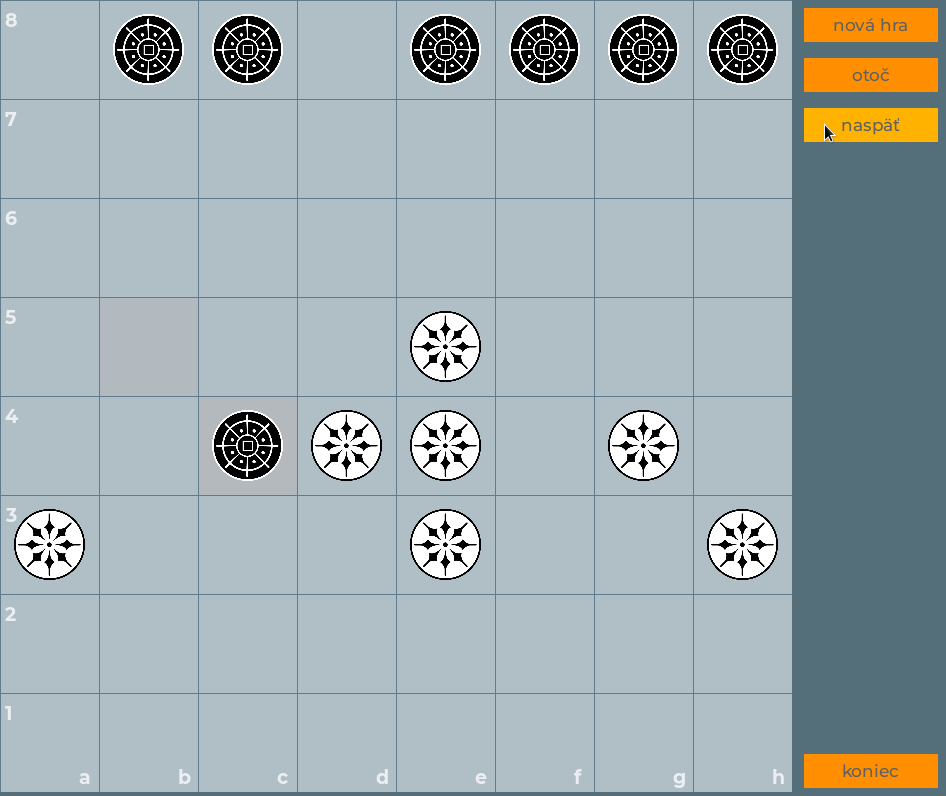
\includegraphics[width=0.55\textwidth]{data/gui.png}}

V našej knižnici bude celé okno rozdelené na {\em widgety}. Widget bude trieda,
ktorá spravuje časť okna, vie sa prispôsobiť zmenenej veľkosti, vie reagovať na
kliknutia myšou (prípadne iné udalosti, napr. stlačenie klávesy) a vie sa
vykresliť do SDL renderera. Príkladom widgetu je naša trieda \vb{BoardView} z
kapitoly~\ref{sect:SDL}. Iný widget by mohol byť napr. \vb{Button}, ktorý predstavuje 
jeden gombík a stará sa o to, aby sa naňho dalo kliknúť. Ďalší typ widgetov sa stará o rozmiestňovanie iných widgetov.
Widget \vb{Layout} si pamätá zoznam widgetov a prepočítava ich veľkosť a umiestnenie.
V našom prípade chceme mať ako hlavný widget horizontálny layout, ktorý obsahuje dva widgety:
\vb{BoardView} a vertikálny layout. Ten obsahuje päť widgetov: tri gombíky, 
jeden widget na vyplnenie miesta a ďalší gombík. 

Takže stačí napísať pre každý widget príslušnú triedu, poskladať to celé dokopy a hotovo.
Vidno tu ale dva problémy. Po prvé, je veľa funkcionality, ktorá je pre všetky (prípadne niektoré)
widgety spoločná. Napr. každý widget si má pamätať \vb{SDL\_Rect rect}, ktorý na obrazovke zaberá.
Takisto môže mať okraje nejakej hrúbky. Takže všetky widgety budú mať metódu 
\hbox{\vb{resize(SDL\_Rect newRect)}}, v ktorej bude

\begin{lstlisting}
  rect = newRect;
  rect.x += padding;
  rect.y += padding;
  rect.w -= 2 * padding;
  rect.h -= 2 * padding;
\end{lstlisting}

Navyše widgety \vb{Layout} ešte prerátajú rozmery svojich vnútorných widgetov a zavolajú
ich \vb{resize}. Postupne sa bude nabaľovať viac a viac kódu, ktorý je na veľa miestach rovnaký,
čo je oštara. Na druhý problém narazíš, ak začneš rozmýšľať, ako naprogramovať typ \vb{Layout}.
Potrebuje mať totiž zoznam svojich vnútorných widgetov, ktoré môžu byť rôznych typov. 
Ukážem ti, že na oba tieto problémy je dobré riešenie mechanizmus, ktorému sa v C++
hovorí {\em dedičnosť}.

Opäť poďme od začiatku. Dajme tomu, že by si mal triedu

\begin{lstlisting}
struct Widget {
  int x, y;
  void render();
};
\end{lstlisting}

Keď urobíš premennú \vb{Widget w}, v pamäti to bude vyzerať takto:

\begin{tikzpicture}[
    boxnode/.style={font=\robotomono,draw, minimum width = 5cm},
    popis/.style ={,anchor=east, left=5mm of #1}
  ]
  \def\nxtnd[#1](#2)(#3)#4{%
  \node[boxnode,#1,rect={#1}{}{#1}{#1}, below = 0cm of #2] (#3)  {#4};
  }

  \node[boxnode,rect={}{}{}{}] (pamat) at (0,0) {dáta};
  \node[boxnode,rect={black}{}{black}{black}, below = 0cm of pamat] (start) { };
  \nxtnd[black](start)(x){int Widget::x}
  \nxtnd[black](x)(y){int Widget::y}
  \node[boxnode,rect={black}{}{black}{}, below = 0cm of y] { };

  \node[popis={x}] (w) {{\robotomono w}};  \draw[->, shorten >= 2ex] (w) -- (x);

  \node[black,boxnode,rect={}{}{}{}] (prog0) at (8,0) {program};
  \node[boxnode,rect={black}{}{black}{black}, below = 0cm of prog0] (ps) { };
  \nxtnd[black](ps)(f){Widget::render()}
  \node[boxnode,rect={black}{}{black}{}, below = 0cm of f] { };
\end{tikzpicture}

To znamená, že každá premenná typu \vb{Widget} má v pamäti dve premenné \vb{int}
a navyše je v programe funkcia \vb{Widget::render()}.\indexItem{Prg}{dedenie}
Teraz môžeš urobiť triedu \vb{Button}, ktorá bude mať všetko to, čo \vb{Widget}
a aj niečo navyše. Hovoríme, že \vb{Button} dedí od \vb{Widget} a zapíše sa to takto:

\begin{lstlisting}
struct Button : Widget {
  string label;
  void render();
  void click();
};
\end{lstlisting}

Každá premenná typu \vb{Button} bude mať tri premenné: dve zdedené od \vb{Widget}
a jednu novú. V programe budú tri funkcie, takže \vb{Button b;} bude vyzerať takto:

\begin{tikzpicture}[
    boxnode/.style={font=\robotomono,draw, minimum width = 5cm},
    popis/.style ={,anchor=east, left=5mm of #1}
  ]
  \def\nxtnd[#1](#2)(#3)#4{%
  \node[boxnode,#1,rect={#1}{}{#1}{#1}, below = 0cm of #2] (#3)  {#4};
  }

  \node[boxnode,rect={}{}{}{}] (pamat) at (0,0) {dáta};
  \node[boxnode,rect={black}{}{black}{black}, below = 0cm of pamat] (start) { };
  \nxtnd[black](start)(x){int Widget::x}
  \nxtnd[black](x)(y){int Widget::y}
  \nxtnd[teal](y)(label){string Button::label}
  \node[boxnode,rect={black}{}{black}{}, below = 0cm of label] { };

  \node[popis={x}] (b) {{\robotomono b}};  \draw[->, shorten >= 2ex] (b) -- (x);

  \node[black,boxnode,rect={}{}{}{}] (prog0) at (8,0) {program};
  \node[boxnode,rect={black}{}{black}{black}, below = 0cm of prog0] (ps) { };
  \nxtnd[black](ps)(f){Widget::render()}
  \nxtnd[teal](f)(g){Button::render()}
  \nxtnd[teal](g)(h){Button::click()}
  \node[boxnode,rect={black}{}{black}{}, below = 0cm of h] { };
\end{tikzpicture}

Môžeš si to vyskúšať, program

\begin{lstlisting}[label={l:ded.1}]
#include <iostream>
#include <string>
using namespace std;

struct Widget {
  int x, y;
  void render() { cout << "Widget::render " << x << " " << y << endl; }
};

struct Button : Widget {
  string label;
  void render() { cout << "Button::render " << x << " " << y << " " << label << endl; } @\ll1@
  void click() { cout << "Button::click " << x << " " << y << " " << label << endl; }
};

int main() {
  Widget w; 
  w.x = 12; w.y = 42; w.render();

  Button b;
  b.x = 17; b.y = 47; b.label = "kikirikí"; b.render(); b.click();
}
\end{lstlisting}

vypíše 

\begin{outputBox}
Widget::render 12 42
Button::render 17 47 kikirikí
Button::click 17 47 kikirikí
\end{outputBox}

Teraz z programu vymaž riadok~\ref{l:ded.1-1}, 
teda v programe už nebude funkcia \vb{Button::render()}. Mala by sa vypísať chyba, že 
\vb{b.render()} volá neexistujúcu funkciu \vb{Button::render()}, ale chyba sa nevypíše.
Keď upravený program spustíš, vypíše sa

\begin{outputBox}
Widget::render 12 42
Widget::render 17 47
Button::click 17 47 kikirikí
\end{outputBox}

Čo sa stalo? Pri dedení sa totiž dedia nielen premenné, ale aj funkcie. Je to podobne ako
s lokálnymi premennými: ak existuje funkcia z daného typu (napr. \vb{Button::render()}),
použije sa tá. Ak neexistuje, kompilátor sa skúsi pozrieť na typ, z ktorého sa dedilo,
a použije funkciu odtiaľ
(napr. \vb{Widget::render()}). Keď sa nad tým zamyslíš, dáva to zmysel: pretože
\vb{Button} obsahuje všetky premenné, ktoré má \vb{Widget}, tak každá funkcia, ktorá
by pracovala na premennej typu \vb{Widget} môže rovnako dobre pracovať na premennej
typu \vb{Button}. V programe sa preto zavolala funkcia \vb{Widget::render()} na
premennú \vb{b}.

Teraz by sa zdalo, že to ale nesedí: v kapitole~\ref{sect:stack} sme hovorili, 
že metódy sú funkcie, ktoré majú ``neviditeľný'' prvý parameter \vb{this}, takže 
v našom prípade máme funkcie

\begin{lstlisting}
void Widget::render (Widget* this) {...}
void Button::render (Button* this) {...}
\end{lstlisting}

Keď sa teda zavolá \vb{Widget::render} namiesto \vb{Button::render}, tak sa 
musí aj zmeniť typ pointra z \vb{Button*} na \vb{Widget*}. To sa aj v skutočnosti udeje
a nielen pri volaní metód. Opäť, keď sa nad tým zamyslíš, tak \vb{Widget*} je
\cmd{adresa v pamäti, kde sa začínajú dáta nejakej premennej typu {\robotomono Widget}}.
To isté ale platí aj pre \vb{Button*}: je to adresa v pamäti, kde sa začínajú dáta
pre nejakú premennú typu \vb{Widget}. Že za nimi sa potom nachádzajú ďalšie dáta tak,
že je to celá premenná typu \vb{Button}, to je už druhá vec.
Preto je vždy možné pointer na ``väčší'' typ (napr. \vb{Button}) použiť tam, kde
sa vyžaduje pointer na ``menší'' typ (napr. \vb{Layout}).

Zase si to vyskúšaj. Vráť naspäť vymazaný riadok tak, aby \vb{Widget} aj \vb{Button}
mali vlastnú funkciu \vb{render} a hlavný program zmeň takto:

\begin{lstlisting}[label={l:ded.2}]
int main() {
  Button *b = new Button;
  b->x = 17;  b->y = 47; b->label = "kikirikí";
  b->render(); @\ll1@

  Widget *q = b; @\ll2@
  q->render(); @\ll3@
}
\end{lstlisting}

Vypíše sa

\begin{outputBox}
Button::render 17 47 kikirikí
Widget::render 17 47
\end{outputBox}

Prečo? Premenná \vb{b} je typu \vb{Button*}, preto volanie \vb{b->render()} na 
riadku~\ref{l:ded.2-1} zavolá funkciu \vb{Button::render}.
Premenná \vb{q} je typu \vb{Widget*}. Na riadku~\ref{l:ded.2-2} sa do nej priradí 
\vb{b}, takže \vb{q} ukazuje na to isté miesto v pamäti, kde je uložená premenná \vb{*b}.
Volanie \vb{q->render()} na riadku~\ref{l:ded.2-3} preto zavolá \vb{Widget::render}
na premennej typu \vb{Widget}, ktorá vznikne ``orezaním'' \vb{*b} do typu \vb{Widget}
(t.j. zabudne sa na \vb{b->label}).

S týmto mechanizmom máme jednu dobrú a jednu zlú správu. Dobrá správa je, že v našom type
\vb{Layout} by sme vedeli spraviť pole rôznych widgetov. Ak všetky widgety budú nejakým 
spôsobom\footnote{aj nepriamo, napr. \vb{Layout} bude dediť z \vb{Widget} a \vb{HLayout}
bude dediť z \vb{Layout}}
dediť zo základného typu \vb{Widget} tak môžeme spraviť \vb{vector<Widget *> children},
ktorý bude obsahovať pointre na widgety, ktoré môžu byť gombíky, ďalšie layouty a pod.

Zlá správa je, že ak potom zavoláme napr.

\begin{lstlisting}
  for (int i = 0; i < children.size(); i++) 
    children[i]->render();
\end{lstlisting}

Tak sa na každé z detí zavolá \vb{Widget::render}. Všetky sú totiž typu \vb{Widget*}
a kompilátor nemá ako vedieť, že kedysi dávno sme tam priradili iné typy. 
Chcelo by to nejaký mechanizmus, ktorým by sa zapamätalo, aký typ má ktoré z detí, aby potom
sa volala metóda \vb{render} z príslušného typu. \indexItem{Prg}{virtuálne metódy}
Tento mechanizmus sa volá {\em virtuálne metódy}. 
Zober si takto zmenenú triedu (pred deklaráciu \vb{render}
som pridal slovo \vb{virtual})

\begin{lstlisting}
struct Widget {
  int x, y;
  virtual void render();
};

void Widget::render() { cout << "Widget::render " << x << " " << y << endl; }
\end{lstlisting}

Keď teraz vyrobíš premennú \vb{Widget w}, v pamäti to bude vyzerať takto:

\begin{tikzpicture}[
    boxnode/.style={font=\robotomono,draw, minimum width = 5cm},
    popis/.style ={,anchor=east, left=5mm of #1}
  ]
  \def\nxtnd[#1](#2)(#3)#4{%
  \node[boxnode,#1,rect={#1}{}{#1}{#1}, below = 0cm of #2] (#3)  {#4};
  }

  \node[boxnode,rect={}{}{}{}] (pamat) at (0,0) {dáta};
  \node[boxnode,rect={black}{}{black}{black}, below = 0cm of pamat] (start) { };
  \nxtnd[orange](start)(vt){Widget::\_vptr}
  \nxtnd[black](vt)(x){int Widget::x}
  \nxtnd[black](x)(y){int Widget::y}
  \node[boxnode,rect={black}{}{black}{}, below = 0cm of y] { };

  \node[popis={vt}] (w) {{\robotomono w}};  \draw[->, shorten >= 2ex] (w) -- (vt);

  \node[orange,boxnode,rect={}{}{}{}] (vt0) at (8,0) {Widget vtable};
  \node[boxnode,rect={}{}{}{orange}, below = 0cm of vt0] (vtr) {};
  \nxtnd[orange](vtr)(vf){typeInfo}
  \nxtnd[orange](vf)(vg){render()}

  \draw[orange, ->,  shorten >= 1ex, shorten <= 1ex] (vt.east) -- (vf.west);
  
  \node[black,boxnode,rect={}{}{}{}] (prog0) at (0,-4) {program};
  \node[boxnode,rect={black}{}{black}{black}, below = 0cm of prog0] (ps) { };
  \nxtnd[black](ps)(f){Widget::render()}
  \node[boxnode,rect={black}{}{black}{}, below = 0cm of f] { };

  \draw[dashed, orange, -> ,shorten >= 1ex, shorten <= 1ex] (vg.west) to [out=180,in=0]  (f.east);
\end{tikzpicture}

Kompilátor pre každý typ, ktorý obsahuje virtuálne metódy, vyrobí v pamäti zoznam \vb{vtable}, kde sú adresy, na ktorých sú v programe uložené príslušné funkcie.
Každá premenná má naviac jednu položku \vb{\_vptr}, čo je pointer 
do \vb{vtable} svojho typu. Virtuálna funkcia, napr. \vb{w.render()} sa teraz nezavolá priamo, ale 
prečíta sa adresa z \vb{vtable} a zavolá sa príslušná funkcia z nej. Akonáhle je nejaká metóda virtuálna, tak sú virtuálne aj všetky jej verzie v zdedených typoch.
Preto keď teraz urobíš

\begin{lstlisting}
struct Button : Widget {
  string label;
  void render();
};

void Button::render() {
  cout << "Button::render " << x << " " << y << " " << label << endl;
}
\end{lstlisting}

tak premenná \vb{Button b} bude v pamäti vyzerať


\begin{tikzpicture}[
    boxnode/.style={font=\robotomono,draw, minimum width = 5cm},
    popis/.style ={,anchor=east, left=5mm of #1}
  ]
  \def\nxtnd[#1](#2)(#3)#4{%
  \node[boxnode,#1,rect={#1}{}{#1}{#1}, below = 0cm of #2] (#3)  {#4};
  }

  \node[boxnode,rect={}{}{}{}] (pamat) at (0,0) {dáta};
  \node[boxnode,rect={black}{}{black}{black}, below = 0cm of pamat] (start) { };
  \nxtnd[orange](start)(vt){Widget::\_vptr}
  \nxtnd[black](vt)(x){int Widget::x}
  \nxtnd[black](x)(y){int Widget::y}
  \nxtnd[teal](y)(z){int Button::label}
  \node[boxnode,rect={black}{}{black}{}, below = 0cm of z] { };

  \node[popis={vt}] (w) {{\robotomono b}};  \draw[->, shorten >= 2ex] (w) -- (vt);

  \node[orange,boxnode,rect={}{}{}{}] (vt0) at (8,0) {Widget vtable};
  \node[boxnode,rect={}{}{}{orange}, below = 0cm of vt0] (vtr) {};
  \nxtnd[orange](vtr)(vf){typeInfo}
  \nxtnd[orange](vf)(vg){render()}

  \node[teal,boxnode,rect={}{}{}{}] (bt0) at (8,-3) {Button vtable};
  \node[boxnode,rect={}{}{}{teal}, below = 0cm of bt0] (btr) {};
  \nxtnd[teal](btr)(bf){typeInfo}
  \nxtnd[teal](bf)(bg){render()}

  \draw[teal, ->,  shorten >= 1ex, shorten <= 1ex] (vt.east) -- ++(1,0) |- (bf.west);
  
  \node[black,boxnode,rect={}{}{}{}] (prog0) at (0,-4) {program};
  \node[boxnode,rect={black}{}{black}{black}, below = 0cm of prog0] (ps) { };
  \nxtnd[black](ps)(f){Widget::render()}
  \nxtnd[black](f)(g){Button::render()}
  \node[boxnode,rect={black}{}{black}{}, below = 0cm of g] { };
  
  \draw[dashed, orange, -> ,shorten >= 1ex, shorten <= 1ex] (vg.west) to [out=180,in=0]  (f.east);
  \draw[dashed, teal, -> ,shorten >= 1ex, shorten <= 1ex] (bg.west) to [out=180,in=0]  (g.east);
\end{tikzpicture}

Typ \vb{Button} zdedil všetky premenné z \vb{Layout} a začiatok pamäte vyzerá rovnako
ako v \vb{Layout}, iba tentokrát \vb{\_vptr} ukazuje na \vb{vtable}, ktorá patrí \vb{Button}.
Teraz je jasné, čo sa stane, ak priradíš napr. \hbox{\vb{Widget *w = \&b;}}
Pointer \vb{w} bude ukazovať na to isté miesto, kde je
uložená \vb{b}, ale keďže je typu \vb{Widget*}, bude ``vidieť'' iba \vb{\_vptr}, \vb{x} a \vb{y}. 
Pointer \vb{\_vptr} bude ale ukazovať na \vb{vtable} pre typ \vb{Button}, preto \vb{w->render()} zavolá 
\hbox{\vb{Button::render()}.}

Takže si to zhrňme. Ak máš rodičovskú triedu (napr. \vb{Layout}), môžeš z nej zdediť triedu pomocou dvojbodky

\begin{lstlisting}
struct Button : Widget { ... };
\end{lstlisting}

Zdedená trieda bude obsahovať všetky premenné a metódy (funkcie) z pôvodnej. Môže si pridať nové premenné a nové metódy s novým menom, prípadne 
predefinovať existujúce (napr. náš \vb{Button::render()}). Pointer na zdedenú triedu sa dá použiť 
všade tam, kde sa vyžaduje pointer na pôvodnú triedu.
Ak je metóda označená ako \vb{virtual}, každá premenná si pamätá, s akým typom bola vytvorená
a vždy zavolá metódu z toho typu.

Pripomínam, že vždy môžeš používať celé meno metódy s dvoma dvojbodkami, aby si rozlíšil, ktorý typ
chceš použiť. Veľakrát chceš urobiť niečo takéto:

\begin{lstlisting}
void Button::render() {
  Widget::render();
  ...
}
\end{lstlisting}

To znamená, že \vb{Button::render()} (ktorý má ``neviditeľný'' prvý parameter \vb{Button *this})
najprv zavolá \hbox{\vb{Widget::render(this)}.} To môže urobiť, lebo \vb{Widget::render} chce parameter
\vb{this} typu \vb{Widget *} a 
\vb{Button} je zdedený z \vb{Widget}. Takže ak zavoláš \vb{b.render()} na premennú
typu \vb{Button}, najprv sa na premennej \vb{b} zavolá \vb{Widget::render()} (ktorá môže
robiť spoločné veci, napr. prekresliť pozadie a pod.) a potom sa urobia veci špecifické pre \vb{Button}.

\indexItem{Prg}{volanie konštruktorov pri dedení}
Tento mechanizmus volania ``rodičovskej'' metódy je trochu iný pri konštruktoroch. Konštruktor
sa totiž zavolá vtedy, keď sa premenná vyrába, a potom ho už nemôžeš volať ``ručne''. Pri zdedených
trieda sa automaticky volajú konštruktory v poradí dedenia, takže v našom prípade by sa najprv
zavolal konštruktor pre \vb{Widget} a po ňom konštruktor pre \vb{Button} (pri deštruktoroch je to 
v opačnom poradí). Preto tento program\footnote{%
  Deštruktor som napísal ako \vb{virtual}. Teraz na tom nezáleží, ale ak máš v triede
  virtuálne metódy, je spravidla dobrý nápad, aby bol aj deštruktor virtuálny. Skús si rozmyslieť,
  prečo.
}:

\begin{lstlisting}
#include <iostream>
using namespace std;

struct Widget {
  Widget() { cout << "Widget constructor" << endl; }
  virtual ~Widget() { cout << "Widget destructor" << endl; }
};

struct Button : Widget {
  Button() { cout << "Button constructor" << endl; }
  virtual ~Button() { cout << "Button destructor" << endl; }
};

int main() {
  Button b;
  cout << "kváák" << endl;
}
\end{lstlisting}

vypíše 

\begin{outputBox}
Widget constructor
Button constructor
kváák
Button destructor
Widget destructor
\end{outputBox}

Ak chceš do konštruktora poslať parametre, dá sa to urobiť pomocou volania koštruktora rodičovskej
triedy za dvojbodkou
rovnako, ako sme volali konštruktory premenných v kapitole~\ref{sect:cukor}.
Vyskúšaj si takto upravený program:

\begin{lstlisting}
#include <iostream>
using namespace std;

struct Widget {
  int x;
  Widget(int _x) : x(_x) { cout << "Widget constructor" << endl; }
  virtual ~Widget() { cout << "Widget destructor" << endl; }
};

struct Button : Widget {
  int y;
  Button(int _x, int _y) : Widget(_x), y(_y) {
    cout << "Button constructor" << endl;
  }
  virtual ~Button() { cout << "Button destructor" << endl; }
};

int main() {
  Button b(42, 47);
  cout << "kváák " << b.x << " " << b.y << endl;
}
\end{lstlisting}

Konštruktor \vb{Button} dostane dva parametre. 
Najprv zavolá konštruktor pre \vb{Widget} s parametrom \vb{\_x}. Ten nastaví\footnote{%
  využil som, že \vb{int} má v C++ aj konštruktor s jedným parametrom
} hodnotu premennej 
\vb{x}. V konštruktore pre \vb{Button} sa potom
premenná \vb{y} nastaví na hodnotu \vb{\_y} a vypíše sa oznam.

Toto je zhruba všetko, čo budeme o dedičnosti potrebovať vedieť do nášho GUI. Nestarali sme sa
tu o riadenie prístupu, len poviem, že privátne premenné a metódy nie sú po dedení viditeľné. Ak by bola
v predchádzajúcom príklade premenná \vb{x} vo \vb{Widget} označená ako \vb{private}, tak 
pri volaní \vb{b.x} vyhlási kompilátor chybu. Ničmenej, premenná \vb{b} by obsahovala aj \vb{x},
ale jediný spôsob, ako sa k nemu \vb{b} môže dostať, je pomocou metód zdedených z \vb{Widget}.

Na riadenie prístupu existujú rôzne módy dedenia, takže niekedy môžeš vidieť napr.
\prg!struct Button : private Widget {...};!, prípadne namiesto \vb{private} môže byť
\vb{public} alebo \hbox{\vb{protected}.} My to tu nebudeme používať, ale ak sa s tým stretneš, 
kompletné detaily sú napr. \link{https://en.cppreference.com/w/cpp/language/derived_class}{tu}.

No a nakoniec len pridám, že je možné dediť aj z viacerých tried. Keby si mal napr. 
triedu \vb{Textual} pre veci obsahujúce text, mohol by si triedu \vb{Button} deklarovať

\begin{lstlisting}
struct Button : Widget, Textual { ... };
\end{lstlisting}

čím by zdedil všetky premenné aj metódy z oboch tried. Niekedy sa to hodí, ale môže to začať
byť trochu komplikované, ak si nedáš pozor. Opäť to tu nebudeme rozoberať, ak ťa to zaujíma,
skús si vyhľadať ``{\em multiple inheritance}'' a ``{\em diamond problem}''.

Vráťme sa teraz k nášmu projektu. Základná trieda \vb{Widget} by mohla vyzerať takto:

\begin{lstlisting}
struct Widget {
  static SDL_Point mouse;

  SDL_Rect rect;
  int fixedHeight = 0;
  int fixedWidth = 0;
  int padding = 0;

  virtual ~Widget(){}

  virtual void resize(SDL_Rect _rect);
  virtual void render(SDL_Renderer *r){}
  virtual void onMouseMotion(SDL_MouseMotionEvent& e){}
  virtual void onMouseDown(SDL_MouseButtonEvent& e){}
  virtual void onMouseUp(SDL_MouseButtonEvent& e){}
};
\end{lstlisting}

Máme statickú premennú \vb{mouse}, do ktorej v hlavnom programe pri spracovaní udalostí zapíšeme
polohu myši. Každý widget má vlastný obdĺžnik \vb{rect}, ktorý zaberá na obrazovke a okraj \vb{padding}.
Môže mať nastavený \vb{fixedWidht} alebo \vb{fixedHeight}, vtedy má vždy danú veľkosť (napr. výška
gombíka je vždy rovnaká). Ak nie sú nastavené, tak sa v danom smere môže naťahovať.

Všetky metódy tu majú prázdne telo: funkcionalita bude až v zdedených triedach. Výnimkou je \vb{resize},
ktorá nastaví obdĺžnik zmenšený o okraje takto:

\begin{lstlisting}
void Widget::resize(SDL_Rect _rect) {
  rect = _rect;
  rect.x += padding;
  rect.y += padding;
  rect.w -= 2 * padding;
  rect.h -= 2 * padding;
}
\end{lstlisting}

Ďalej si spravíme triedu \vb{Layout} a z nej zdedené triedy \vb{VLayout} a \vb{HLayout}:

\vbox{
\begin{lstlisting}
struct Layout : Widget {
  std::vector<Widget *> children;
  std::vector<SDL_Rect> rects;

  ~Layout();
  void render(SDL_Renderer *r);

  Layout& operator<<(Widget *w);  // pridá w na koniec children

  void onMouseMotion(SDL_MouseMotionEvent& e);
  void onMouseDown(SDL_MouseButtonEvent& e);
  void onMouseUp(SDL_MouseButtonEvent& e);
};

struct HLayout : Layout {
  void resize(SDL_Rect _rect);
};

struct VLayout : Layout {
  void resize(SDL_Rect _rect);
};
\end{lstlisting}
}

\vb{Layout} si pamätá zoznam detí a obdĺžnikov, ktoré zaberajú. Všetky metódy \vb{Layout}
len zavolajú príslušné metódy detí, napr.

\begin{lstlisting}
void Layout::onMouseDown(SDL_MouseButtonEvent &e) {
  for (auto &c : children)
    if (SDL_PointInRect(&mouse, &(c->rect))) c->onMouseDown(e);
}
\end{lstlisting}

Hlavnú prácu robia zdedené  \vb{VLayout::resize()} a \vb{HLayout::resize()}, ktoré
na základe celého obdĺžnika prerátajú obdĺžniky detí: tie, ktoré majú fixný rozmer, nechajú fixný
a ostatné rovnomerne rozdelia medzi zvyšok. Nakoniec sa zavolá

\begin{lstlisting}
for (int i = 0; i < children.size(); i++) children[i]->resize(rects[i]);
\end{lstlisting}

Tu je treba sa rozhodnúť, kto bude ``vlastniť'' widgety v layoute. Inými slovami, kto je
zodpovedný za to, aby sa správne zmazali, keď ich už netreba. Ja som sa rozhodol, že 
ich bude vlastniť layout, to znamená, že deštruktor layoutu zavolá deštruktory detí. 
Potom si treba ustrážiť, aby sa už inde v programe widgety, ktoré sa pridajú do layoutu,
nemazali.

Ešte budeme potrebovať gombíky, napr.

\begin{lstlisting}
struct Button : Widget {
  static TTF_Font *font;
  Text label, labelDisabled;
  std::string txt;
  bool clicked;
  bool disabled;
  std::function<void(void)> onClick = [](){};

  SDL_Color bgNormal, bgHovered, bgClicked, bgDisabled, fgNormal, fgDisabled;

  Button(const std::string &_txt=" ");

  void render(SDL_Renderer *r);
  void onMouseMotion(SDL_MouseMotionEvent& e);
  void onMouseDown(SDL_MouseButtonEvent& e);
  void onMouseUp(SDL_MouseButtonEvent& e);
};
\end{lstlisting}

Gombík si pamätá, či sa naňho práve kliklo (\vb{onMouseDown} nastaví \vb{clicked} na \vb{true}
a \vb{onMouseUp} na \vb{false}) a či nie je vypnutý a podľa toho sa pri volaní \vb{render}
vykreslí. Navyše má premennú \vb{onClick}, čo je lambda, ktorá sa zavolá, keď sa
na gombík klikne.

\begin{uloha}
  Urob program pre \btr, ktorý vyzerá ako screenshot na začiatku tejto kapitoly:
  má gombíky na novú hru, vrátenie ťahu, otočenie šachovnice a skončenie programu.
\end{uloha}

Ak si prišiel až sem, gratulujem. Napísal si celkom veľký, použiteľný program. Určite máš veľa
nápadov, ako by sa dal vylepšiť. Pri programoch tejto veľkosti (a väčších)
je najväčšia zábava, ak sa spojíte viacerí a skúsite všetky svoje nápady spoločne realizovať.

